This is the first module in our pipeline, its responsibility is to get the textual description of the image from speech. It takes the speech as input then processes it to get its textual content to be used to extract the facial features used to generate the image.

\subsubsection{Functional Description}

Our aim is to add functionality that the user can enter a speech description of the image to generate it, so we used an automatic speech recognition model based on \texttt{DeepSpeech2} \cite{amodei2015deep}, we used the Spectograms features from the audio and applied some preprocessing to those features before training. The target of the speech model is to detect the English spoken words and get their textual meaning so that it can be used to generate the Face Image and output the desired described Face.

\begin{itemize}
    \item \textbf{Input :}
    \begin{itemize}
        \item Speech audio wave.
    \end{itemize}
    \item \textbf{Output :}
    \begin{itemize}
        \item The spoken words on the input audio (textual description).
    \end{itemize}
\end{itemize}

\subsubsection{Modular Decomposition}

\begin{figure}[H]
    \centering
    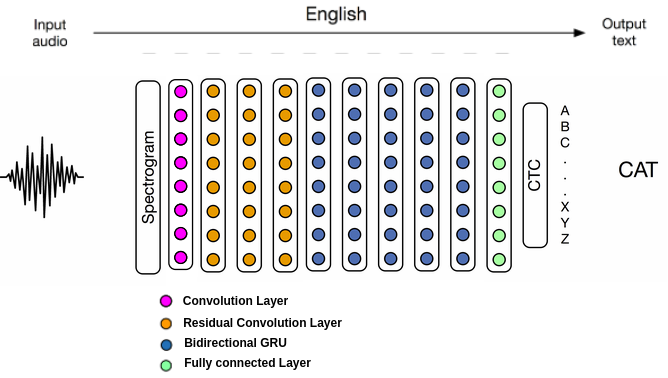
\includegraphics[width=0.8\textwidth]{images/speech.png}
    \caption{Modified DeepSpeech2 network architecture.}
    \label{fig:speechModel}
\end{figure}

As mentioned, we use \texttt{DeepSpeech2} with connectionist temporal classification (CTC) losses as a base to our speech recognition model. The model takes as input features from the audio in the form of spectrograms compressed by frequency and time masking to separate the spectrograms in time and frequency domains. \\
The model architecture (shown in figure \ref{fig:speechModel}) consists of one convolutional layer followed by 3 residual CNNs and 5 bidirectional gated recurrent units GRUs. \\

The first convolution layer used to compress the audio information in low dimension space, The residual CNN consists of layer normalization over the time axis of the speech then 2 convolution layers summed with the original input to the resCNN. \\

The bidirectional RNN uses 512 hidden units used to predict the input character at each time step, The last layer is a fully connected layer to out the final predicted character for each input spectrogram. \\

Connectionist Temporal Classification (CTC) loss function is used to align each character and its location in the audio input file, By summing the probabilities of possible alignments of the input to target and producing a loss value which is differentiable with respect to the model inputs and functions weights. After that those weights are updated using Adam optimizer to minimize this loss value until convergence. \\
\begin{equation}
    L(x,y;\theta) = - \log \sum_{l 	\in Align(x,y)}^{} \prod_{t}^{T} pctc (l_{t} |x;\theta )
\end{equation}

The best aligned character is selected using greedy beam search from all available character to the corresponding input. \\ 
The model Was trained and tested on LibriSpeech ASR corpus which consists of 100 hours for training and test set, "clean" speech for testing. We calculate the word error rate (WER) and character error rate (CER) for the test data to evaluate the model performance.


\subsubsection{Design Constraints}

As our application is a real time interactive app, It’s a must for the speech recognition model to be very fast to be able to process the input quickly so that we gain the users satisfaction. It was a constraint as we couldn't  use larger model with more accurate results, as it will increase the processing time which is against our needs.

